\chapter{Resultados}
En el capítulo anterior describimos el proceso para segmentar las imágenes a través del canal Hue. Empleando diferentes valores para los parámetros de umbral inferior y umbral superior (\Cref{sec:segmentation}) se obtienen los siguientes resultados.

\section{Segmentación Hue en 40 y 120}
\begin{table}[H]
\centering
\begin{tabular}{|l|l|l|l|l|}
\hline 
\textbf{Clasificación} & \textbf{Total} & \textbf{Aciertos} & \textbf{Errores} & \textbf{Eficiencia} \\
\hline
Estado & 1393 & 962 & 431 & 69.059 \\
\hline 
Categoría & 1393 & 715 & 678 & 51.328 \\
\hline 
\end{tabular}
\caption{Eficiencias generales con Hue 40-120}
\label{table:efficiency_general_40_120}
\end{table}

\captionsetup[figure]{skip=-10pt}

\begin{figure}[H]
\centering
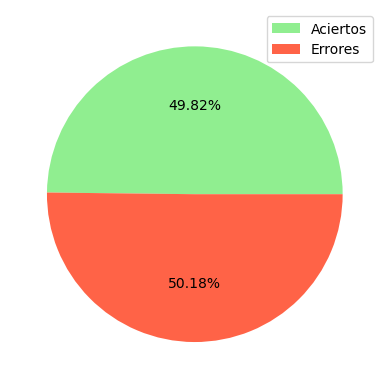
\includegraphics[scale=0.6]{images/result_global_state_40_120.png}
\caption{Eficiencia detectando el estado con Hue 40-120}
\label{img:efficiency_state_40_120}
\end{figure}

\begin{figure}[H]
\centering
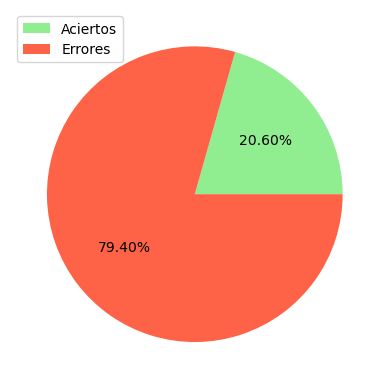
\includegraphics[scale=0.6]{images/result_global_class_40_120.png}
\caption{Eficiencia detectando la categoría con Hue 40-120}
\label{img:efficiency_category_40_120}
\end{figure}

\captionsetup[figure]{skip=10pt}

\begin{table}[H]
\centering
\begin{tabular}{|l|c|c|c|}
\hline 
\textbf{Categoría} & \textbf{Original} & \textbf{Calculado} & \textbf{Eficiencia} \\
\hline
healthy & 791 & 445 & 56.257 \\
\hline 
rust\_level\_1 & 344 & 196 & 56.976 \\
\hline 
rust\_level\_2 & 166 & 67 & 40.361 \\
\hline 
rust\_level\_3 & 62 & 6 & 9.677 \\
\hline 
rust\_level\_4 & 30 & 1 & 3.333 \\
\hline 
\end{tabular}
\caption{Eficiencia por categoría con Hue 40-120}
\label{table:efficiency_categories_40_120}
\end{table}

\begin{figure}[H]
\centering
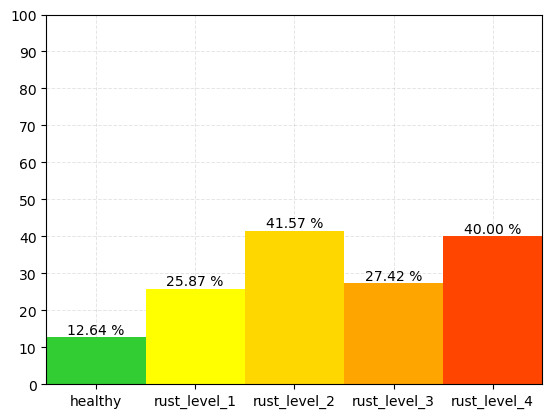
\includegraphics[scale=0.6]{images/result_classes_40_120.png}
\caption{Eficiencia por categoría con Hue 40-120}
\label{img:efficiency_categories_40_120}
\end{figure}


\section{Segmentación Hue en 40 y 80}
\begin{table}[h!]
\centering
\begin{tabular}{|l|l|l|l|l|}
\hline 
\textbf{Clasificación} & \textbf{Total} & \textbf{Aciertos} & \textbf{Errores} & \textbf{Eficiencia} \\
\hline
Estado & 1393 & 962 & 431 & 69.059 \\
\hline 
Categoría & 1393 & 715 & 678 & 51.328 \\
\hline 
\end{tabular}
\caption{Eficiencias generales con Hue 40-80}
\label{table:efficiency_general_40_80}
\end{table}

\captionsetup[figure]{skip=-10pt}

\begin{figure}[H]
\centering
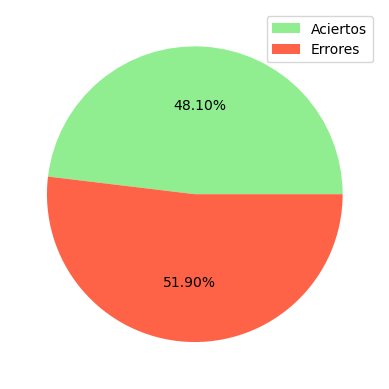
\includegraphics[scale=0.6]{images/result_global_state_40_80.png}
\caption{Eficiencia detectando el estado con Hue 40-80}
\label{img:efficiency_state_40_80}
\end{figure}

\begin{figure}[H]
\centering
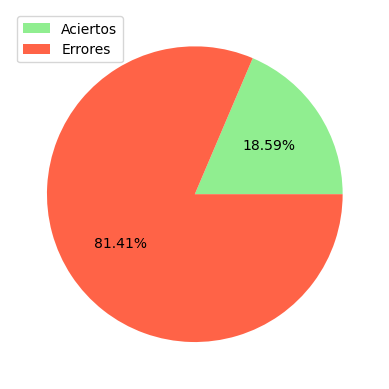
\includegraphics[scale=0.6]{images/result_global_class_40_80.png}
\caption{Eficiencia detectando la categoría con Hue 40-80}
\label{img:efficiency_category_40_80}
\end{figure}

\captionsetup[figure]{skip=10pt}

\begin{table}[h!]
\centering
\begin{tabular}{|l|c|c|c|}
\hline 
\textbf{Categoría} & \textbf{Original} & \textbf{Calculado} & \textbf{Eficiencia} \\
\hline
healthy & 791 & 445 & 56.257 \\
\hline 
rust\_level\_1 & 344 & 196 & 56.976 \\
\hline 
rust\_level\_2 & 166 & 67 & 40.361 \\
\hline 
rust\_level\_3 & 62 & 6 & 9.677 \\
\hline 
rust\_level\_4 & 30 & 1 & 3.333 \\
\hline 
\end{tabular}
\caption{Eficiencia por categoría con Hue 40-80}
\label{table:efficiency_categories_40_80}
\end{table}

\begin{figure}[H]
\centering
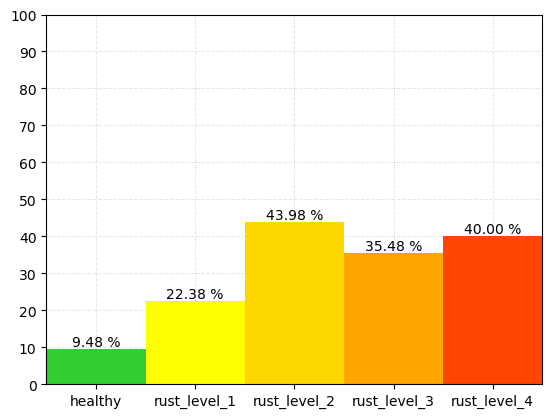
\includegraphics[scale=0.6]{images/result_classes_40_80.png}
\caption{Eficiencia por categoría con Hue 40-80}
\label{img:efficiency_categories_40_80}
\end{figure}


\section{Segmentación Hue en 30 y 120}
La \Cref{table:efficiency_general_30_120} muestra el porcentaje de eficiencia alcanzado para clasificar las hojas de café por su estado saludable o infectado (\Cref{img:efficiency_state_30_120}), o bien, el porcentaje de eficiencia global para las categorías (\Cref{img:efficiency_category_30_120}).

\begin{table}[h!]
\centering
\begin{tabular}{|l|l|l|l|l|}
\hline 
\textbf{Clasificación} & \textbf{Total} & \textbf{Aciertos} & \textbf{Errores} & \textbf{Eficiencia} \\
\hline
Estado & 1393 & 962 & 431 & 69.059 \\
\hline 
Categoría & 1393 & 715 & 678 & 51.328 \\
\hline 
\end{tabular}
\caption{Eficiencias generales con Hue 30-120}
\label{table:efficiency_general_30_120}
\end{table}

\captionsetup[figure]{skip=-10pt}

\begin{figure}[H]
\centering
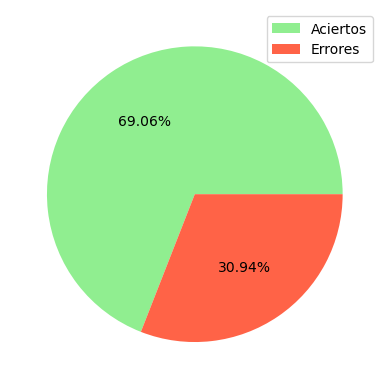
\includegraphics[scale=0.6]{images/result_global_state_30_120.png}
\caption{Eficiencia detectando el estado con Hue 30-120}
\label{img:efficiency_state_30_120}
\end{figure}

\begin{figure}[H]
\centering
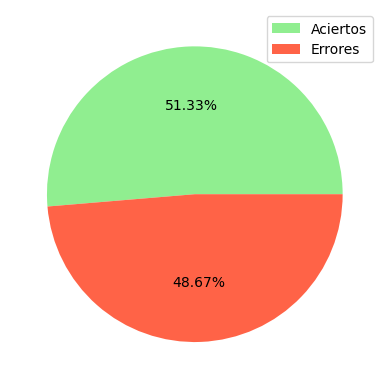
\includegraphics[scale=0.6]{images/result_global_class_30_120.png}
\caption{Eficiencia detectando la categoría con Hue 30-120}
\label{img:efficiency_category_30_120}
\end{figure}

\captionsetup[figure]{skip=10pt}

A su vez la \Cref{table:efficiency_categories_30_120} muestra la eficiencia alcanzada por cada una de las categorías: saludable, roya nivel 1, roya nivel 2, roya nivel 3 y roya nivel 4 (\Cref{img:efficiency_categories_30_120}).

\begin{table}[h!]
\centering
\begin{tabular}{|l|c|c|c|}
\hline 
\textbf{Categoría} & \textbf{Original} & \textbf{Calculado} & \textbf{Eficiencia} \\
\hline
healthy & 791 & 445 & 56.257 \\
\hline 
rust\_level\_1 & 344 & 196 & 56.976 \\
\hline 
rust\_level\_2 & 166 & 67 & 40.361 \\
\hline 
rust\_level\_3 & 62 & 6 & 9.677 \\
\hline 
rust\_level\_4 & 30 & 1 & 3.333 \\
\hline 
\end{tabular}
\caption{Eficiencia por categoría con Hue 30-120}
\label{table:efficiency_categories_30_120}
\end{table}

\begin{figure}[H]
\centering
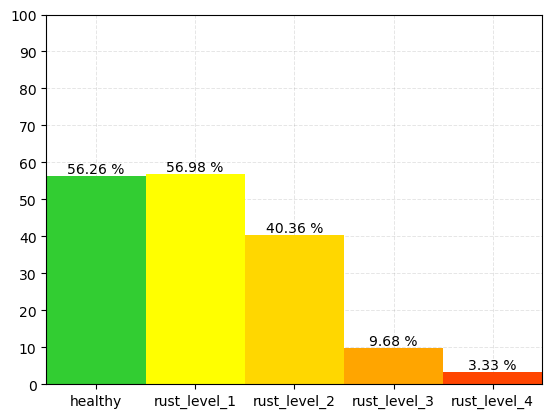
\includegraphics[scale=0.6]{images/result_classes_30_120.png}
\caption{Eficiencia por categoría con Hue 30-120}
\label{img:efficiency_categories_30_120}
\end{figure}


\section{Segmentación Hue en 30 y 100}
\begin{table}[h!]
\centering
\begin{tabular}{|l|l|l|l|l|}
\hline 
\textbf{Clasificación} & \textbf{Total} & \textbf{Aciertos} & \textbf{Errores} & \textbf{Eficiencia} \\
\hline
Estado & 1393 & 962 & 431 & 69.059 \\
\hline 
Categoría & 1393 & 715 & 678 & 51.328 \\
\hline 
\end{tabular}
\caption{Eficiencias generales con Hue 30-100}
\label{table:efficiency_general_30_100}
\end{table}

\captionsetup[figure]{skip=-10pt}

\begin{figure}[H]
\centering
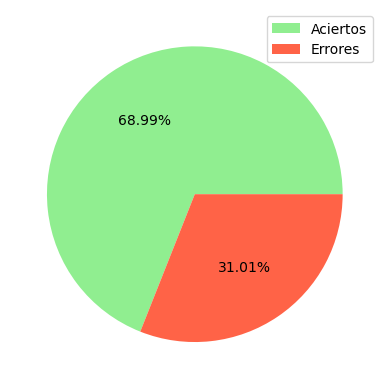
\includegraphics[scale=0.6]{images/result_global_state_30_100.png}
\caption{Eficiencia detectando el estado con Hue 30-100}
\label{img:efficiency_state_30_100}
\end{figure}

\begin{figure}[H]
\centering
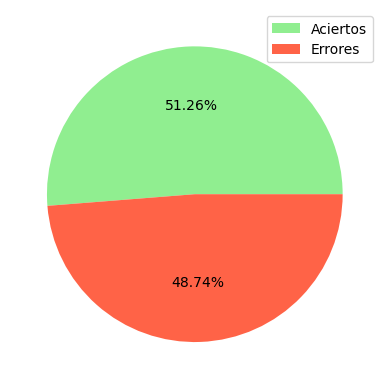
\includegraphics[scale=0.6]{images/result_global_class_30_100.png}
\caption{Eficiencia detectando la categoría con Hue 30-100}
\label{img:efficiency_category_30_100}
\end{figure}

\captionsetup[figure]{skip=10pt}

\begin{table}[h!]
\centering
\begin{tabular}{|l|c|c|c|}
\hline 
\textbf{Categoría} & \textbf{Original} & \textbf{Calculado} & \textbf{Eficiencia} \\
\hline
healthy & 791 & 445 & 56.257 \\
\hline 
rust\_level\_1 & 344 & 196 & 56.976 \\
\hline 
rust\_level\_2 & 166 & 67 & 40.361 \\
\hline 
rust\_level\_3 & 62 & 6 & 9.677 \\
\hline 
rust\_level\_4 & 30 & 1 & 3.333 \\
\hline 
\end{tabular}
\caption{Eficiencia por categoría con Hue 30-100}
\label{table:efficiency_categories_30_100}
\end{table}

\begin{figure}[H]
\centering
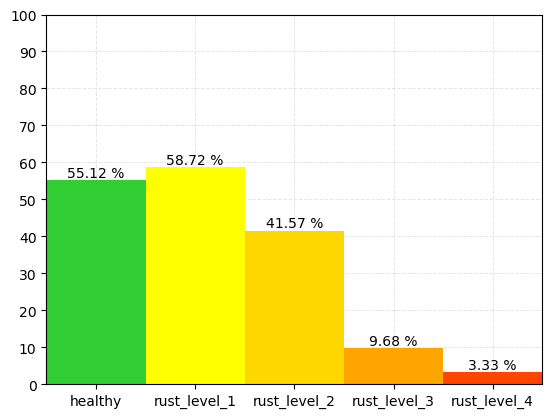
\includegraphics[scale=0.6]{images/result_classes_30_100.png}
\caption{Eficiencia por categoría con Hue 30-100}
\label{img:efficiency_categories_30_100}
\end{figure}


\section{Segmentación Hue en 30 y 80}
\begin{table}[h!]
\centering
\begin{tabular}{|l|l|l|l|l|}
\hline 
\textbf{Clasificación} & \textbf{Total} & \textbf{Aciertos} & \textbf{Errores} & \textbf{Eficiencia} \\
\hline
Estado & 1393 & 962 & 431 & 69.059 \\
\hline 
Categoría & 1393 & 715 & 678 & 51.328 \\
\hline 
\end{tabular}
\caption{Eficiencias generales con Hue 30-80}
\label{table:efficiency_general_30_80}
\end{table}

\captionsetup[figure]{skip=-10pt}

\begin{figure}[H]
\centering
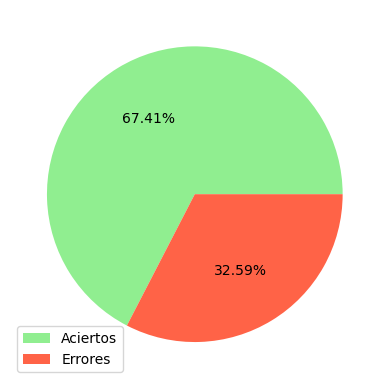
\includegraphics[scale=0.6]{images/result_global_state_30_80.png}
\caption{Eficiencia detectando el estado con Hue 30-80}
\label{img:efficiency_state_30_80}
\end{figure}

\begin{figure}[H]
\centering
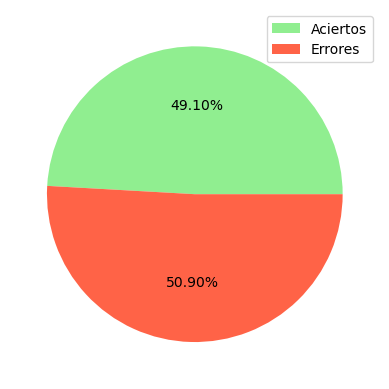
\includegraphics[scale=0.6]{images/result_global_class_30_80.png}
\caption{Eficiencia detectando la categoría con Hue 30-80}
\label{img:efficiency_category_30_80}
\end{figure}

\captionsetup[figure]{skip=10pt}

\begin{table}[h!]
\centering
\begin{tabular}{|l|c|c|c|}
\hline 
\textbf{Categoría} & \textbf{Original} & \textbf{Calculado} & \textbf{Eficiencia} \\
\hline
healthy & 791 & 445 & 56.257 \\
\hline 
rust\_level\_1 & 344 & 196 & 56.976 \\
\hline 
rust\_level\_2 & 166 & 67 & 40.361 \\
\hline 
rust\_level\_3 & 62 & 6 & 9.677 \\
\hline 
rust\_level\_4 & 30 & 1 & 3.333 \\
\hline 
\end{tabular}
\caption{Eficiencia por categoría con Hue 30-80}
\label{table:efficiency_categories_30_80}
\end{table}

\begin{figure}[H]
\centering
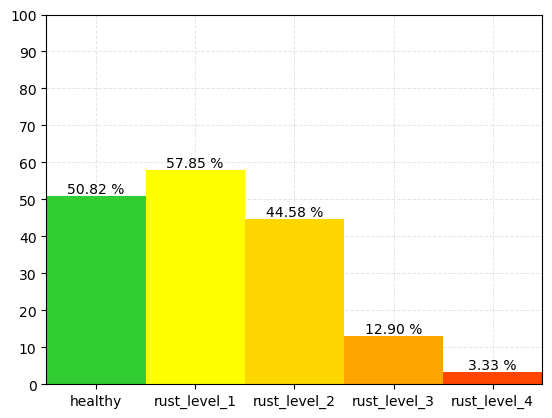
\includegraphics[scale=0.6]{images/result_classes_30_80.png}
\caption{Eficiencia por categoría con Hue 30-80}
\label{img:efficiency_categories_30_80}
\end{figure}


\section{Segmentación Hue en 28 y 120}
La \Cref{table:efficiency_general_28_120} muestra el porcentaje de eficiencia alcanzado para clasificar las hojas de café por su estado saludable o infectado (\Cref{img:efficiency_state_28_120}), o bien, el porcentaje de eficiencia global para las categorías (\Cref{img:efficiency_category_28_120}).

\begin{table}[h!]
\centering
\begin{tabular}{|l|l|l|l|l|}
\hline 
\textbf{Clasificación} & \textbf{Total} & \textbf{Aciertos} & \textbf{Errores} & \textbf{Eficiencia} \\
\hline
Estado & 1393 & 962 & 431 & 69.059 \\
\hline 
Categoría & 1393 & 715 & 678 & 51.328 \\
\hline 
\end{tabular}
\caption{Eficiencias generales con Hue 28-120}
\label{table:efficiency_general_28_120}
\end{table}

\captionsetup[figure]{skip=-10pt}

\begin{figure}[!ht]
\centering
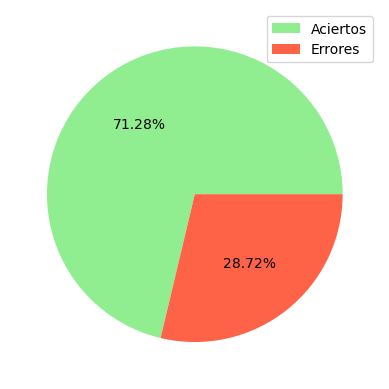
\includegraphics[scale=0.6]{images/result_global_state_28_120.png}
\caption{Eficiencia detectando el estado con Hue 28-120}
\label{img:efficiency_state_28_120}
\end{figure}

\begin{figure}
\centering
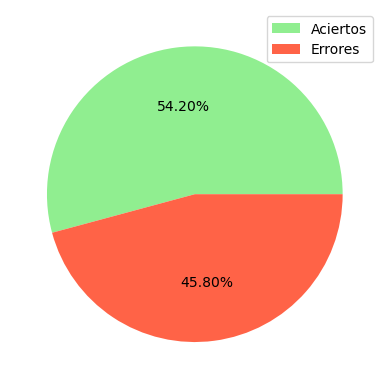
\includegraphics[scale=0.6]{images/result_global_class_28_120.png}
\caption{Eficiencia detectando la categoría con Hue 28-120}
\label{img:efficiency_category_28_120}
\end{figure}

\captionsetup[figure]{skip=10pt}

A su vez la \Cref{table:efficiency_categories_28_120} muestra la eficiencia alcanzada por cada una de las categorías: saludable, roya nivel 1, roya nivel 2, roya nivel 3 y roya nivel 4 (\Cref{img:efficiency_categories_28_120}).

\begin{table}[h!]
\centering
\begin{tabular}{|l|c|c|c|}
\hline 
\textbf{Categoría} & \textbf{Original} & \textbf{Calculado} & \textbf{Eficiencia} \\
\hline
healthy & 791 & 445 & 56.257 \\
\hline 
rust\_level\_1 & 344 & 196 & 56.976 \\
\hline 
rust\_level\_2 & 166 & 67 & 40.361 \\
\hline 
rust\_level\_3 & 62 & 6 & 9.677 \\
\hline 
rust\_level\_4 & 30 & 1 & 3.333 \\
\hline 
\end{tabular}
\caption{Eficiencia por categoría con Hue 28-120}
\label{table:efficiency_categories_28_120}
\end{table}

\begin{figure}
\centering
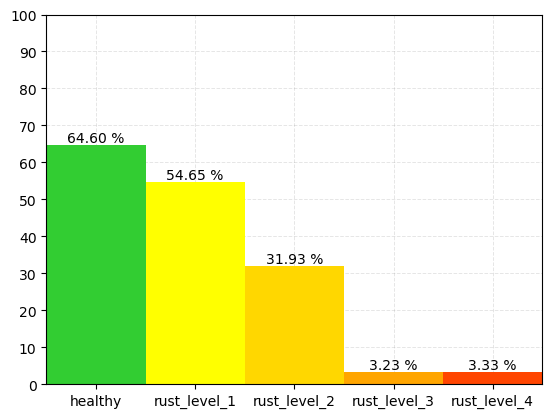
\includegraphics[scale=0.6]{images/result_classes_28_120.png}
\caption{Eficiencia por categoría con Hue 28-120}
\label{img:efficiency_categories_28_120}
\end{figure}


\section{Segmentación Hue en 25 y 120}
La \Cref{table:efficiency_general_25_120} muestra el porcentaje de eficiencia alcanzado para clasificar las hojas de café por su estado saludable o infectado (\Cref{img:efficiency_state_25_120}), o bien, el porcentaje de eficiencia global para las categorías (\Cref{img:efficiency_category_25_120}).

\begin{table}[h!]
\centering
\begin{tabular}{|l|l|l|l|l|}
\hline 
\textbf{Clasificación} & \textbf{Total} & \textbf{Aciertos} & \textbf{Errores} & \textbf{Eficiencia} \\
\hline
Estado & 1393 & 962 & 431 & 69.059 \\
\hline 
Categoría & 1393 & 715 & 678 & 51.328 \\
\hline 
\end{tabular}
\caption{Eficiencias generales con Hue 25-120}
\label{table:efficiency_general_25_120}
\end{table}

\captionsetup[figure]{skip=-10pt}

\begin{figure}[H]
\centering
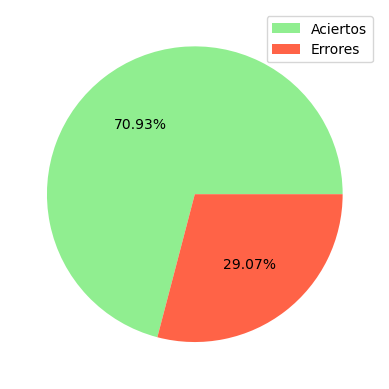
\includegraphics[scale=0.6]{images/result_global_state_25_120.png}
\caption{Eficiencia detectando el estado con Hue 25-120}
\label{img:efficiency_state_25_120}
\end{figure}

\begin{figure}
\centering
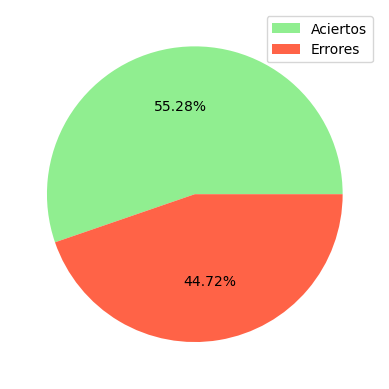
\includegraphics[scale=0.6]{images/result_global_class_25_120.png}
\caption{Eficiencia detectando la categoría con Hue 25-120}
\label{img:efficiency_category_25_120}
\end{figure}

\captionsetup[figure]{skip=10pt}

A su vez la \Cref{table:efficiency_categories_25_120} muestra la eficiencia alcanzada por cada una de las categorías: saludable, roya nivel 1, roya nivel 2, roya nivel 3 y roya nivel 4 (\Cref{img:efficiency_categories_25_120}).

\begin{table}[h!]
\centering
\begin{tabular}{|l|c|c|c|}
\hline 
\textbf{Categoría} & \textbf{Original} & \textbf{Calculado} & \textbf{Eficiencia} \\
\hline
healthy & 791 & 445 & 56.257 \\
\hline 
rust\_level\_1 & 344 & 196 & 56.976 \\
\hline 
rust\_level\_2 & 166 & 67 & 40.361 \\
\hline 
rust\_level\_3 & 62 & 6 & 9.677 \\
\hline 
rust\_level\_4 & 30 & 1 & 3.333 \\
\hline 
\end{tabular}
\caption{Eficiencia por categoría con Hue 25-120}
\label{table:efficiency_categories_25_120}
\end{table}

\begin{figure}
\centering
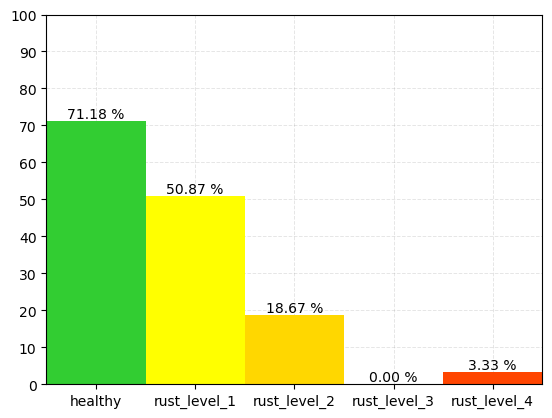
\includegraphics[scale=0.6]{images/result_classes_25_120.png}
\caption{Eficiencia por categoría con Hue 25-120}
\label{img:efficiency_categories_25_120}
\end{figure}


\section{Casos especiales}

\subsection{Iluminación}

\subsection{Envés de la hoja}